
% Третья глава работы 
\chapter{Моделирование систем с алгоритмом RED в NS-2 и Mininet}
\label{chap3}

В данном разделе представлены результаты исследований. Для запуска моделей используем сеть c топологией, представленной в ~\ref{ch3:fig1}.
 
\begin{figure}[h!]
 \centerline{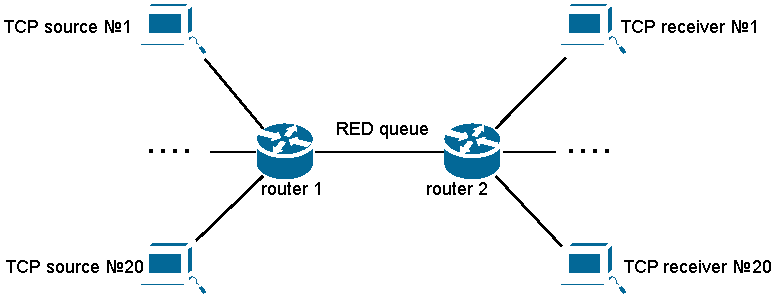
\includegraphics[width=0.7\textwidth]{topology}}
 \caption{Схема топологии моделируемой сети}
\label{ch3:fig1}
\end{figure}

Для данной топологии задали следующие параметры:

\begin{itemize}
\item между TCP-источниками и первым маршрутизатором дуплексные соединения 
	с пропускной способностью 100 Мбит/с и
  	задержкой 20 мс очередью типа DropTail;
\item между TCP-приёмниками и вторым маршрутизатором установлены
  	дуплексные соединения с пропускной способностью 100 Мбит/с и
  	задержкой 20 мс очередью типа DropTail;
\item между маршрутизаторами установлено симплексное соединение
  	($R1$--$R2$) с пропускной способностью 20 Мбит/с и задержкой 15 мс
  	очередью типа RED, размером буфера 300 пакетов; в обратную сторону~---
  	симплексное соединение ($R2$--$R1$) с пропускной способностью 15 Мбит/с и
  	задержкой 20 мс очередью типа DropTail;
\item параметры алгоритма RED: $q_{\min}=75$, $q_{\max}=150$, $q_w=0,002$, $p_{\max}=0.1$;
\item максимальный размер TCP-окна 32; размер передаваемого пакета 1000 байт;
  	байт; время моделирования~---100 единиц модельного времени.
\end{itemize}

\section{Моделирование сети в NS-2}
\label{chap3:sec1}

В имитационной модели TCP-приемники/источники, а также маршрутизаторы реализованы как стандартные узлы, данные передаются по протоколу FTP поверх TCP-Reno, 
для получения данных используются стандартные в программе средства, графики визуализируются в xgraph(для быстрого просмотра) и в GNUPLOT(для дальнейшего анализа).
Модифицированный NS-2 представлен в репозитории ~\cite{ns2-with-red}:


Запустив первую модель с заданными параметрами, получили следующие результаты ~\ref{ch3:fig2}.

\begin{figure}[h!]
 \centerline{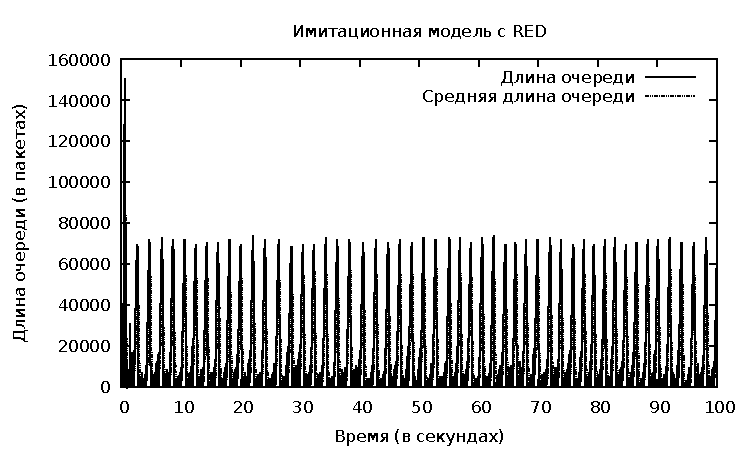
\includegraphics[width=0.7\textwidth]{queues_red}}
 \caption{График длины очереди и средней длины очереди на линке между маршрутизаторами}
\label{ch3:fig2}
\end{figure}


\section{Моделирование сети в Mininet}
\label{chap3:sec2}

Модель в Mininet более сложная в реализации. В нем используются реальные виртуальные маршрутизаторы из класса LinuxRouter, использованы коммутаторы для подсоединения к маршрутизаторам нескольких оконечных устройств, а также настроена ip-адресация для корректной работы программы. Для настройки очереди использован tc в которой реализованы только модийикации RED и ARED, передача пакетов происходит с помощью iperf3 и выводятся в json файл, из которой данные извлекаются с помощью shell скрипта из ~\cite{iperf3-plotter}. Для запуска на нескольких устройствах используются паралельные потоки. Для визуализации также используется GNUPLOT.      

\section{Сравнение результатов в 2 средствах моделирования}
\label{chap3:sec3}

Текст.

%%% Local Variables:
%%% mode: latex
%%% coding: utf-8-unix
%%% TeX-master: "../default"
%%% End:
